% Template for ICASSP-2021 paper; to be used with:
%          spconf.sty  - ICASSP/ICIP LaTeX style file, and
%          IEEEbib.bst - IEEE bibliography style file.
% --------------------------------------------------------------------------
\documentclass{article}
\usepackage{spconf,amsmath,graphicx}
\usepackage{hyperref}
\usepackage{caption}
\usepackage{algorithm,algorithmicx,algpseudocode}
% Example definitions.
% --------------------
\def\x{{\mathbf x}}
\def\L{{\cal L}}


\title{Minimally-Supervised Speech Synthesis with Conditional Diffusion Model and Language Model: A Comparative Study of Semantic Coding}


\name{Chunyu Qiang$^{1,2,*}$, Hao Li$^{2,*}$, Hao Ni$^{2}$, He Qu$^{2}$, Ruibo Fu$^{3}$, Tao Wang$^{3}$, Longbiao Wang$^{1}$, Jianwu Dang$^{1}$}


\address{$^1$College of Intelligence and Computing, Tianjin University, Tianjin, China \\
$^2$Kuaishou Technology Co., Ltd, Beijing, China \\
$^3$Institute of Automation, Chinese Academy of Sciences, Beijing, China 
}



\begin{document}
%\ninept
%
\maketitle
%

% \begin{abstract}
%   We present three speech synthesis systems that combine conditional diffusion models and language models. 1) Diff-LM-Speech: comprehends text-to-speech (TTS) as a fusion of two primary tasks, an autoregressive discrete coding classification task (text into semantic coding) and a non-autoregressive continuous signal prediction task (semantic coding into speech). 2) Tetra-Diff-Speech: treats both tasks as non-autoregressive continuous signal prediction tasks. 3) Tri-Diff-Speech: a non-autoregressive TTS framework based entirely on the diffusion model. Diff-LM-Speech and Tetra-Diff-Speech decouple the training process into supervised and unsupervised components, our method allows for the utilization of abundant audio-only data, thus facilitating training with minimal supervision. Diff-LM-Speech resolves the challenges associated with high dimensionality and waveform distortion in existing autoregressive language modeling methods, while simultaneously addressing the requirement for accurate alignment information in non-autoregressive approaches. Tri-Diff-Speech achieves better diversity and expressiveness in speech synthesis.Experimental results show that the method outperforms the baseline. We provide a website with audio samples. \href{https://qiangchunyu.github.io/style-transfer/STW.html}{$^1$}.

% \end{abstract}
\begin{abstract}
  Recently, there has been a growing interest in text-to-speech (TTS) methods that can be trained with minimal supervision by combining two types of discrete speech representations and using two sequence-to-sequence tasks to decouple TTS. To address the challenges associated with high dimensionality and waveform distortion in discrete representations, we propose Diff-LM-Speech, which models semantic embeddings into mel-spectrogram based on diffusion models and introduces a prompt encoder structure based on variational autoencoders and prosody bottlenecks to improve prompt representation capabilities. Autoregressive language models often suffer from missing and repeated words, while non-autoregressive frameworks face expression averaging problems due to duration prediction models. To address these issues, we propose Tetra-Diff-Speech, which designs a duration diffusion model to achieve diverse prosodic expressions. While we expect the information content of semantic coding to be between that of text and acoustic coding, existing models extract semantic coding with a lot of redundant information and dimensionality explosion. To verify that semantic coding is not necessary, we propose Tri-Diff-Speech. Experimental results show that our proposed methods outperform baseline methods. We provide a website with audio samples. \href{https://qiangchunyu.github.io/Diff-LM-Speech/diff_speech.html}{$^1$}.

\end{abstract}


%

\renewcommand{\thefootnote}{\fnsymbol{footnote}} %将脚注符号设置为fnsymbol类型,即特殊符号表示
\footnotetext[1]{Equal Contribution.} %对应脚注[1]
\footnotetext[2]{Audio samples: https://qiangchunyu.github.io/Diff-LM-Speech/diff\_speech.html}
\footnotetext{Preprint. Work in progress.}

\begin{keywords}
minimal supervision, diversity and expressive speech synthesis, non-autoregressive, diffusion model, language model
\end{keywords}
%
\section{Introduction}
\label{sec:intro}
With the advancement of deep learning, speech synthesis technology has made remarkable progress. Traditional speech synthesis methods have achieved good results on limited datasets\cite{wang2017tacotron,arik2017deep, li2019neural,ren2019fastspeech, kim2020glow, elias2021parallel}. However, the emergence of technologies such as GPT \cite{radford2018improving, brown2020language} has led to an increased interest in large-scale TTS systems.These systems can be broadly classified into two categories, as shown in Fig.1: 1) autoregressive classification tasks based on language models \cite{borsos2022audiolm, wang2023neural,zhang2023speak,kharitonov2023speak}, and 2) non-autoregressive continuous signal regression tasks based on diffusion models \cite{levkovitch2022zero, shen2023naturalspeech, le2023voicebox}.

\begin{figure}[t]
 \centering
 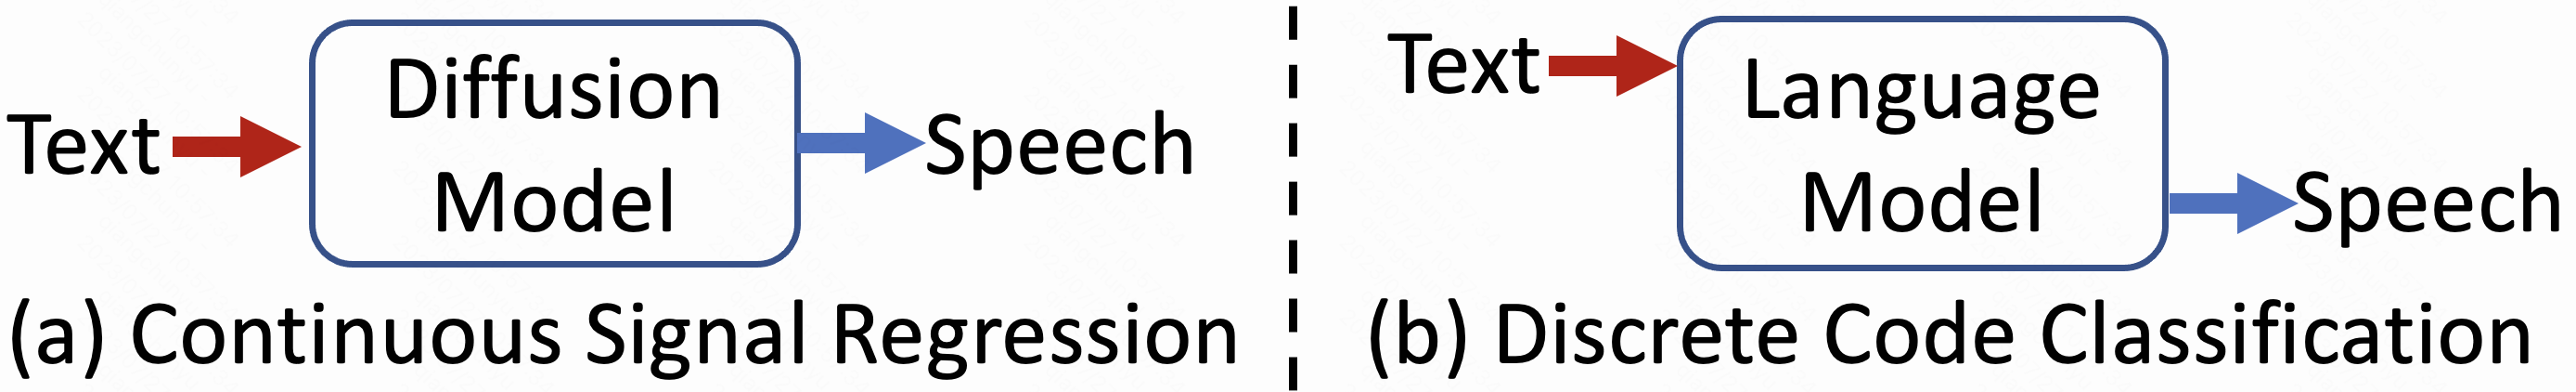
\includegraphics[width=\linewidth]{compare.png}
  \vspace{-15pt}
  \captionsetup{belowskip=-20pt}
 \caption{Existing TTS framework.}
 \label{fig:proposed_model}
\end{figure}


\begin{figure*}[t]
 \centering
 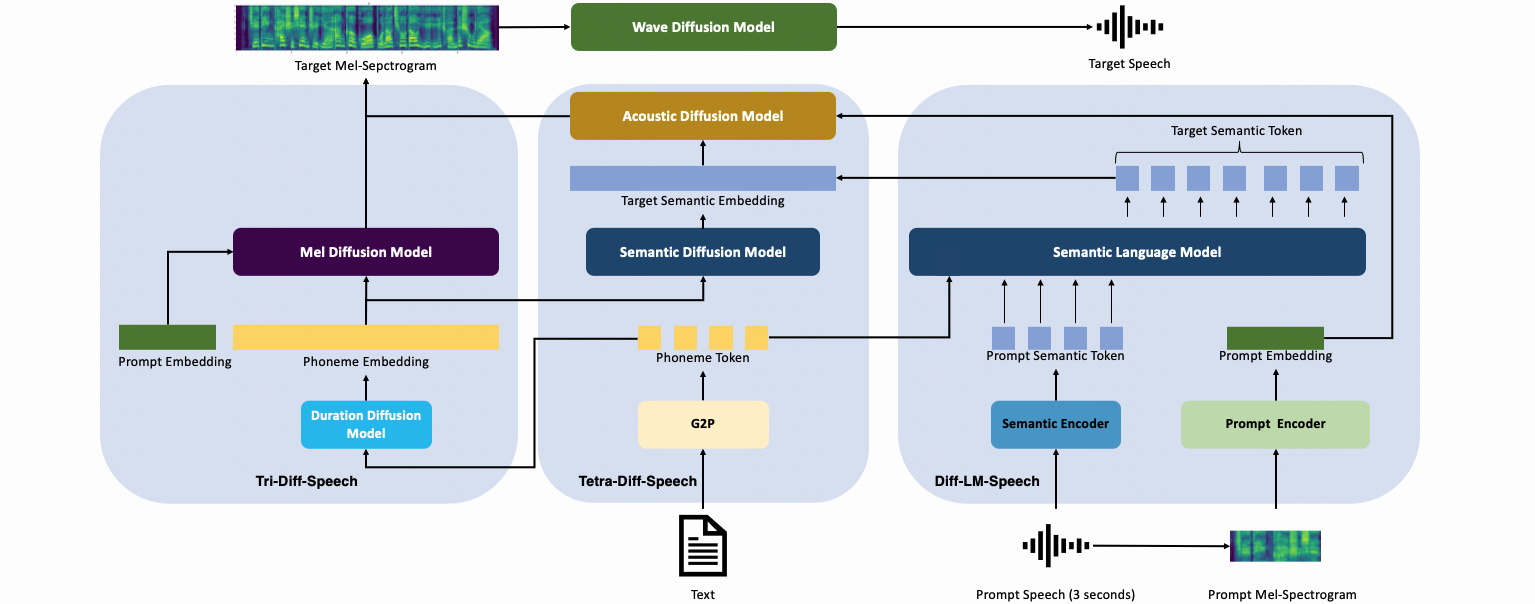
\includegraphics[width=\linewidth]{model.png}
 \vspace{-20pt}
 \captionsetup{belowskip=-20pt}
 \caption{The architecture of proposed model.}
 \label{fig:proposed_model}
\end{figure*}
Traditional speech synthesis methods often use mel-spectrogram as intermediate representations. However, with the recent advancements in neural codec for speech \cite{baevski2020wav2vec, Hsu2021HuBERTSS, Defossez2022HighFN, Zeghidour2022SoundStreamAE}, large-scale TTS methods have started converting audio waveforms into discrete codes as intermediate representations. Some notable examples include VALL-E \cite{wang2023neural}, which is the first large-scale TTS framework based on a language model with in-context learning capabilities and realizes zero-shot speech synthesis, and NaturalSpeech2 \cite{shen2023naturalspeech}, which is a non-autoregressive TTS framework based on latent diffusion model \cite{rombach2022high}. SPEAR-TTS \cite{zhang2023speak} is another example that splits the TTS task into two tasks (text-to-semantic and semantic-to-speech) to realize minimal-supervised training. However, the existing language model-based framework requires the semantic coding and acoustic coding to be discrete. The acoustic coding based on neural codecs for speech waveform reconstruction suffers from information loss on high-frequency fine-grained acoustic details compared to traditional audio features. Additionally, the duration prediction model required by the non-autoregressive framework leads to the problem of expressive averaging. To address these challenges, this paper proposes three novel frameworks:

1) Diff-LM-Speech addresses the issues of high dimensionality and waveform distortion in existing autoregressive language modeling methods. It also avoids the need for precise alignment information in non-autoregressive methods. 
2) Tetra-Diff-Speech designs a duration diffusion model to achieve diverse prosodic expressions. It solves the common problems of missing and repeating words in autoregressive language models, as well as the issue of expressive averaging in non-autoregressive frameworks caused by duration prediction models.
3) Tri-Diff-Speech validates the non-necessity of semantic encoding, avoiding the problem of redundant information and dimension explosion in existing models.




% \begin{itemize}
% \item Diff-LM-Speech is proposed to address the challenges associated with high dimensionality and waveform distortion in existing autoregressive language modeling methods, while simultaneously addressing the requirement for accurate alignment information in non-autoregressive approaches. 


% \item Tetra-Diff-Speech is proposed to validate the comparative effectiveness of the semantic encoding modeling task under autoregressive language models and non-autoregressive diffusion models, both Diff-LM-Speech and Tetra-Diff-Speech are implemented with minimal-supervised training.

% \item Tri-Diff-Speech is proposed to validate the non-necessity of semantic encoding, and a diffusion-based duration prediction model is designed to solve the problem of expressive averaging.
% \end{itemize}








\section{Method}

\subsection{Overview}
% \subsubsection{Diff-LM-Speech}
% Diff-LM-Speech extends SPEAR-TTS\cite{zhang2023speak} by enabling the diffusion model for continuous-valued acoustic feature regression tasks. Diff-LM-Speech is divided into three main stages, as shown in Fig.2. In the first stage, text input is translated into a sequence of discrete semantic tokens by the semantic language model. The second stage maps the semantic embedding into mel-spectrogram by the acoustic diffusion model. The third stage maps mel-spectrogram into speech by the wave diffusion model. Diff-LM-Speech cast text-to-speech (TTS) as a composition of two primary tasks, an autoregressive discrete coding classification task (text into semantic coding) and a non-autoregressive continuous signal prediction task (semantic coding into speech). 


\subsubsection{Diff-LM-Speech}
Diff-LM-Speech extends SPEAR-TTS\cite{zhang2023speak} by enabling the diffusion model for continuous-valued acoustic feature regression tasks. The framework consists of three main stages, as shown in Fig.2. In the first stage, text input is translated into a sequence of discrete semantic tokens by the semantic language model. The second stage maps the semantic embedding into mel-spectrogram by the acoustic diffusion model. The third stage maps mel-spectrogram into speech by the wave diffusion model. Diff-LM-Speech performs two primary tasks: an autoregressive discrete coding classification task (text into semantic coding) and a non-autoregressive continuous signal prediction task (semantic coding into speech).

\subsubsection{Tetra-Diff-Speech}
% As shown in Fig.2, Tetra-Diff-Speech consists of four diffusion-based modules, which differ from Diff-LM-Speech in that a non-autoregressive Semantic Diffusion model is used to achieve the prediction from text to semantic embedding. A duration diffusion model is also designed to predict the corresponding duration of phonemes to solve the problem of mismatch between the length of phoneme sequences and semantic sequences. During training, the ground-truth duration is used to expand the phoneme sequence. During inference, the corresponding predicted duration is used.

Tetra-Diff-Speech, as shown in Fig.2, consists of four diffusion-based modules that differ from Diff-LM-Speech. A non-autoregressive semantic diffusion model is used to achieve the prediction from text to semantic embedding. A duration diffusion model is also designed to predict the corresponding duration of phonemes to solve the problem of mismatch between the length of phoneme sequences and semantic sequences. During training, the ground-truth duration is used to expand the phoneme sequence, while during inference, the corresponding predicted duration is used.


\subsubsection{Tri-Diff-Speech}
% As shown in Fig.2, Tri-Diff-Speech consists of three diffusion-based modules, where the difference with Tetra-Diff-Speech is the use of a Mel Diffusion model to make direct predictions from text to mel-spectrogram, to verify whether the two-stage process based on semantic coding is really effective relative to the traditional one-stage process.

Tri-Diff-Speech, also shown in Fig.2, consists of three diffusion-based modules that use a mel diffusion model to make direct predictions from text to mel-spectrogram. This framework aims to verify whether the two-stage process based on semantic coding is really effective relative to the traditional one-stage process. 

\subsection{Prompt Feature Extractor}
\subsubsection{Semantic Encoder}

Similar to SPEAR-TTS\cite{zhang2023speak}, we use semantic coding as an intermediate representation between text and acoustic coding. To preserve high-frequency fine-grained acoustic details, we replace the discrete acoustic coding generated by SoundStream\cite{zeghidour2021soundstream} with mel-spectrogram. The purpose of semantic coding is to provide coarse, high-level conditioning to subsequently produce mel-spectrogram.  Thus, semantic coding should provide a representation of speech in which linguistic content (phonetics-to-semantics) is salient, while paralinguistic information such as speaker identity and acoustic details are removed. To obtain such a representation(512 dimensions of embedding, 1024 discrete values), we trained a HuBert\cite{hsu2021hubert} model and fine-tuned it on an automatic speech recognition(ASR) task. This approach enables the model to learn a more robust and discriminative representation of speech that captures phonetic and semantic information. Additionally, we used an encoder module of the Whisper\cite{radford2023robust} as a control group to extract semantic coding(512-dimensional).

\subsubsection{Prompt Encoder}

The prompt encoder is a VAE-based model \cite{qiang2023improving} that extracts paralinguistic information, such as timbre, style, and rhyme, from the prompt speech. It comprises a 6-layer 2D convolutional network and a SE-ResNet block \cite{hu2018squeeze}, which recalibrates channel-wise feature responses by modeling interdependencies among channels, resulting in significant performance improvements. The VAE structure enables the model to obtain a continuous and complete latent space distribution of styles, improving the ability to extract paralinguistic information. A 64-dimensional vector is sampled from the Gaussian distribution as the global style embedding. To address the KL collapse problem, three tricks are used: 1) introducing KL annealing, 2) adopting a staged optimization method to optimize the reconstruction loss first and then the KL loss, and 3) A margin $\Delta$ is introduced to limit the minimum value of the kl loss as shown:${L}_{kl} = max(0, D_{KL}[\mathcal{N}({\hat{\mu}},{\hat{\sigma}}^2)||\mathcal{N}(0, I)]-\Delta)$. 

\begin{figure}[t]
 \centering
 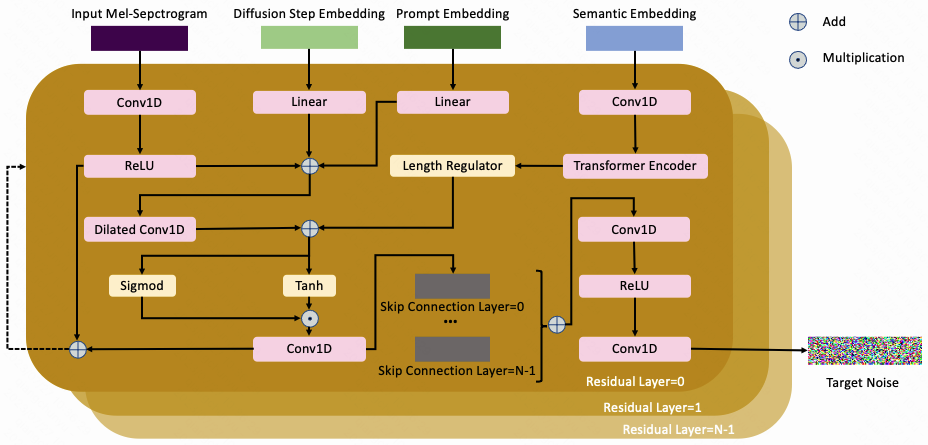
\includegraphics[width=\linewidth]{diffusion.png}
 \vspace{-20pt}
 \captionsetup{belowskip=-15pt}
 
 \caption{The architecture of acoustic diffusion model.}
 \label{fig:proposed_model}
\end{figure}

\subsection{Conditional Diffusion Model}
\subsubsection{Diffusion  Formulation}
The conditional diffusion model involves a diffusion process and a reverse process, with $T$ diffusion steps. The acoustic diffusion model calculation is shown in Algorithm\ref{alg:training} \ref{alg:sampling}. Throughout the paper, we use $q(data), x_0, s, t$ and $p$ to represent data distribution, acoustic coding, semantic coding, diffusion step and prompt embedding, respectively. A notable property of the forward process is that it admits sampling $x_t$ at an arbitrary timestep $t$ in closed form: using the notation $\bar{\alpha}_t$ and $\alpha_t$, we have $x_t = \sqrt{\bar\alpha_t} x_0 + \sqrt{1-\bar\alpha_t}\varepsilon$. $\epsilon_{\theta}$ is a function approximator intended to predict $\epsilon$ from $x_t, t, p$ and $s$. In this paper, we use minimizing the unweighted variant of the ELBO\cite{ho2020denoising} as the training objective, as shown in line 7 of Algorithm\ref{alg:training}.


Algorithm\ref{alg:sampling} shows the sampling process, the generative procedure involves first sampling $x_T \sim \mathcal{N}(0, I)$, and then sampling $x_{t-1}\sim p_{\theta}(x_{t-1}|x_t)$ for $t=T, T-1,\cdots,1$. The reparameterization is shown in line 5 of Algorithm\ref{alg:sampling}. Note that both $\mu_{\theta}$ and $\sigma_{\theta}$ take four inputs: $x_t, t, p$ and $s$. The aim of $p_{\theta}(x_{t-1}|x_t)$ is to eliminate the Gaussian noise added in the diffusion process. The output $x_0$ is the sampled data. 

\subsubsection{Diffusion  Architecture}
In this section, we introduce the architecture of the acoustic diffusion model, which is illustrated in Fig. 3.  It is a non-autoregressive network $\epsilon_{\theta}$ that employs a bidirectional dilated convolution architecture, similar to DiffWave\cite{kong2020diffwave}. The network comprises $N$ residual layers, which are grouped into $m$ blocks, and each containing $n = \frac{N}{m}$ layers. In each layer, we use a dilated convolution with a kernel size of $3$. The dilation is doubled at each layer within each block, i.e., $[1, 2, 4, \cdots, 2^{n-1}]$. We sum the skip connections from all residual layers as in WaveNet\cite{oord2016wavenet}. In the acoustic diffusion model, the conditional information includes semantic embedding and prompt embedding. The semantic embedding is first input to the transformer encoder. Then, it is upsampled by length regulator (transposed 2-D convolutions) to match the length of the mel-spectrogram. Subsequently, it is added as a bias term for the dilated convolution in each residual layer. On the other hand, the prompt embedding and diffusion step embedding are broadcast over length and added to the input of each residual layer.

The other diffusion-based modules have a similar structure, except for the input, diffusion-step and conditional information. As shown in Fig.2, the conditional information of the duration diffusion model(diffusion-step=5) is the phoneme sequence, while the conditional information of the semantic diffusion model(diffusion-step=200) is the phoneme sequence that has been upsampled based on duration. The conditional information of the mel diffusion model(diffusion-step=500) is also the phoneme sequence that has been upsampled based on duration, along with the prompt embedding. Finally, the wave diffusion model(diffusion-step=50) is conditioned on the mel-spectrogram.


\section{Experiments}

\subsection{Experimental Step}
In the experimental step, we utilized the AISHELL-3 dataset\cite{shi2020aishell}, which consists of 88035 recordings of 218 native Mandarin Chinese speakers (43 males and 175 females) reading from given scripts with neutral emotions. All speech waveforms were sampled at 24kHz and converted to mel-spectrograms with a frame size of 960 and a hop size of 240. During the inference phase, we used the centroid of the prompt embeddings extracted from all sentences for each speaker. To simulate a few-shot scenario, we used a test set consisting of 15 minutes and 5 minutes of data for each speaker.


\subsection{Compared Models}
We compared our proposed model with four other models, namely {\bf Tacotron-VAE}\cite{qiang2022style}, {\bf VALL-E}\cite{wang2023neural}, {\bf NaturalSpeech2}\cite{shen2023naturalspeech}, and {\bf SpearTTS}\cite{zhang2023speak}. To ensure fairness, we modified all methods to utilize the same language model and diffusion model framework. Specifically, the prompt encoder, wave diffusion model, and G2P\cite{qiang2022back}  structure of our proposed model were identical across all compared models. The duration diffusion model of both {\bf Tri-Diff-Speech} (described in Sec 2.1.3) and {\bf Tetra-Diff-Speech} (described in Sec 2.1.2) was also the same. Additionally, the semantic encoder and acoustic diffusion model of both {\bf Tetra-Diff-Speech} and {\bf Diff-LM-Speech} (described in Sec 2.1.1) were identical. We used both Hubert and Whisper encoders as control groups for semantic encoding.


\subsection{Test Metrics}
We conducted all subjective tests using 11 native judgers, with each metric consisting of 20 sentences per speaker. The test metrics used in the evaluation included {\bf Prosody Measurement}, which involved mean square error for pitch (MSEP) and duration (MSED) to assess prosody similarity against ground-truth speech, {\bf Word Error Rate(WER)}, which utilized an ASR model to transcribe the generated speech and calculate the word error rate, and {\bf Mean Opinion Score(MOS)}, which verified sound quality and similarity in expected speaking prosody and timbre between source speech and synthesized speech.



\algrenewcommand\algorithmicindent{0.5em}%
\begin{figure}[t]
\begin{minipage}[t]{0.495\textwidth}
\begin{algorithm}[H]
  \caption{Training} \label{alg:training}
  \setlength{\belowdisplayskip}{-10pt}
  \small
  \begin{algorithmic}[1]
    \Repeat
      \State $x_0, s \sim q(data)$
      \State $t \sim \mathrm{Uniform}(\{1, \dotsc, T\})$
      \State $p = {\hat{\mu}} + {\hat{\sigma}} \odot \phi ; \phi \sim \mathcal{N}(0, I)$
      \State $\varepsilon \sim \mathcal{N}(0, I)$
      \State $\bar{\alpha}_t = \prod_{i=1}^t\alpha_i$
      \State Take gradient descent step on
        \Statex $\nabla _\theta \left\| \varepsilon - \varepsilon_\theta((\sqrt{\bar\alpha_t} x_0 + \sqrt{1-\bar\alpha_t}\varepsilon), t, p, s) \right\|^2$
    \Until{converged}
  \end{algorithmic}
\end{algorithm}
\end{minipage}

\hfill
\begin{minipage}[t]{0.495\textwidth}
\begin{algorithm}[H]
  \caption{Sampling} \label{alg:sampling}
  \small
  \begin{algorithmic}[1]
    \vspace{.04in}
    \State $x_T \sim \mathcal{N}(0, I)$
    \For{$t=T, \dotsc, 1$}
      
      \State $\mu_{\theta}(x_t, t, p, s) = \frac{1}{\sqrt{\alpha_t}}\left( x_t - \frac{1-\alpha_t}{\sqrt{1-\bar\alpha_t}} \varepsilon_\theta(x_t, t, p, s) \right)$
      \State $\sigma_{\theta}(x_t, t, p, s) =  \sqrt{\frac{1-\bar{\alpha}_{t-1}}{1-\bar{\alpha}_t}(1-\alpha_t)}$
      
      \State $x_{t-1} = \mu_{\theta} + \sigma_{\theta} \odot \psi; $ $\psi \sim \mathcal{N}(0, I)$ if $t > 1$, else $\psi = 0$
    \EndFor
    \State \textbf{return} $x_0$
    \vspace{.04in}
  \end{algorithmic}
\end{algorithm}
\end{minipage}
\vspace{-1em}
\end{figure}


% \begin{table*}[]
%  \caption{Prosody Measurement \& WER \& MOS}
%  \label{tab:prosody}
%  \centering
% \begin{tabular}{llllll}
% \hline
% Model              & MSEP                    & MSED      & WER      & Prosody Sim           & Speaker Sim           \\ \hline
% Tacotron-VAE\cite{qiang2022style}          & 97.4          & \textbf{18.7} & 7.8            & 3.82 ± 0.072          & 3.92 ± 0.087          \\ \hline
% VALL-E\cite{wang2023neural}                 & 91.6         & 19.5          & 6.1            & 3.64 ± 0.050          & 3.70 ± 0.052          \\ \hline
% NaturalSpeech2\cite{shen2023naturalspeech} & 95.9          & 25.1          & \textbf{4.5}   & 3.73 ± 0.054          & 4.04 ± 0.086          \\ \hline
% SpearTTS(Hubert)\cite{zhang2023speak}      & 110.5         & 19.0          & 8.5            & 3.60 ± 0.059          & 3.68 ± 0.030          \\ \hline
% Tetra-Diff-Speech(Hubert)                                   & 103.5         & 20.1          & 4.6         & 3.89 ± 0.013          & 3.71 ± 0.077          \\ \hline
% Tetra-Diff-Speech(Whisper)                                  & 104.4         & 21.2          & 4.6          & 3.79 ± 0.098          & 3.93 ± 0.057          \\ \hline
% Diff-LM-Speech(Hubert)                                      & 107.2         & 19.6          & 7.2          & 3.80 ± 0.090          & 3.71 ± 0.015          \\ \hline
% Diff-LM-Speech(Whisper)                                     & 107.0         & \textbf{18.7} & 7.7          & 3.80 ± 0.064          & 3.79 ± 0.044          \\ \hline
% Tri-Diff-Speech                                             & \textbf{95.2} & 19.0          & \textbf{4.5}  & \textbf{3.90 ± 0.047} & \textbf{4.06 ± 0.010} \\ \hline
% \end{tabular}
% \end{table*}






\subsection{Results}
The results in Table 1 demonstrate that one-stage models, including Tri-Diff-Speech, NaturalSpeech2, VALLE-E, and Tacotron-VAE, outperform two-stage models like Spear-TTS, Tetra-Diff-Speech, and Diff-LM-Speech in terms of MSEP. Additionally, we observed that existing models extract redundant information and cause dimensionality explosion in semantic coding, making overall task modelling more challenging than one-stage modelling. Due to the limited number of open-source Mandarin datasets, we plan to further verify this conclusion in future work. In terms of MSED, Diff-LM-Speech achieves the best results, while Tri-Diff-Speech and Tetra-Diff-Speech also perform better than the non-autoregressive structure of NaturalSpeech2 due to the duration diffusion model. Furthermore, Tri-Diff-Speech and NaturalSpeech2 have significant advantages over other autoregressive structures (VALL-E, Diff-LM-Speech, etc.) in synthesizing high-quality and robust speech due to their non-autoregressive structure, as demonstrated by the WER results.


Table 2 reveals that the proposed methods outperform SpearTTS, NaturalSpeech2, and VALL-E in terms of prosody similarity MOS, thanks to the duration diffusion model. Among them, Tri-Diff-Speech achieves the best results. For speaker similarity MOS, both Tri-Diff-Speech and NaturalSpeech2 with non-autoregressive structure perform better. Moreover, all models using mel-spectrogram as acoustic features achieve better sound quality MOS scores than those with discrete acoustic coding. Specifically, Tri-Diff-Speech and Tacotron-VAE achieve the best results, highlighting the importance of continuous acoustic features for sound quality.


\begin{table}[]
\captionsetup{skip=5pt} % 设置标题与表格之间的间距为10pt
 \caption{Prosody Measurement \& WER}
 \label{tab:prosody}
 \centering
 \resizebox{\linewidth}{!}{ 
\begin{tabular}{llll}
\hline
Model              & MSEP                    & MSED      & WER      \\ \hline
Tacotron-VAE\cite{qiang2022style}          & 97.4          & \textbf{18.7} & 7.8          \\ \hline
VALL-E\cite{wang2023neural}                 & 98.6         & 19.5          & 6.1         \\ \hline
NaturalSpeech2\cite{shen2023naturalspeech} & 95.9          & 25.1          & \textbf{4.5} \\ \hline
SpearTTS(Hubert)\cite{zhang2023speak}      & 110.5         & 19.0          & 8.5          \\ \hline
Tetra-Diff-Speech(Hubert)                                   & 103.5         & 20.1          & 4.6          \\ \hline
Tetra-Diff-Speech(Whisper)                                  & 104.4         & 21.2          & 4.6          \\ \hline
Diff-LM-Speech(Hubert)                                      & 107.2         & \textbf{18.7}          & 7.2          \\ \hline
Tri-Diff-Speech                                             & \textbf{95.2} & 19.0          & \textbf{4.5} \\ \hline
\end{tabular}
}
\end{table}

\begin{table}[]
\captionsetup{skip=5pt} % 设置标题与表格之间的间距为10pt
 \caption{MOS}
 \label{tab:mos}
 \centering
\resizebox{\linewidth}{!}{ 
\begin{tabular}{llll}
\hline
Model                      & Prosody Sim           & Speaker Sim           & Sound Quality         \\ \hline
Tacotron-VAE               & 3.82 ± 0.072          & 3.92 ± 0.087          & \textbf{4.01 ± 0.023}          \\ \hline
VALL-E                     & 3.64 ± 0.050          & 3.70 ± 0.052          & 3.61 ± 0.013          \\ \hline
NaturalSpeech2             & 3.73 ± 0.054          & 4.04 ± 0.086          & 3.79 ± 0.070          \\ \hline
SpearTTS(Hubert)           & 3.60 ± 0.059          & 3.68 ± 0.030          & 3.50 ± 0.081          \\ \hline
Tetra-Diff-Speech(H)  & 3.89 ± 0.013          & 3.71 ± 0.077          & 4.00 ± 0.002          \\ \hline
Tetra-Diff-Speech(W) & 3.79 ± 0.098          & 3.93 ± 0.057          & 3.99 ± 0.017          \\ \hline
Diff-LM-Speech(H)     & 3.80 ± 0.090          & 3.71 ± 0.015          & 3.88 ± 0.042          \\ \hline
Tri-Diff-Speech            & \textbf{3.90 ± 0.047} & \textbf{4.06 ± 0.010} & \textbf{4.01 ± 0.080} \\ \hline
\end{tabular}
}
\end{table}

\section{Conclusions}
In this paper, Diff-LM-Speech, Tetra-Diff-Speech and Tri-Diff-Speech are proposed. We address the problem of high dimensionality and waveform distortion due to discrete coding by modeling semantic embeddings into mel-spectrogram based on diffusion models. More diverse, high-quality and robust speech synthesis is achieved by the proposed multiple methods. The non-essentiality of the two-stage model (based on semantic coding) is also verified. Experiments show the effectiveness of the proposed methods. 

\vfill\pagebreak





\bibliographystyle{IEEEbib}

\footnotesize
\bibliography{strings,refs}




\end{document}


